%To determine the whether using OSKI would be beneficial to applications at Sandia we ran
%tests on representative matrices and machines in common use at Sandia.
To assess the potential benefit of using OSKI in Sandia applications, we ran tests on representative
data and a variety of advanced architectures.  For these tests OSKI version 1.0.1h was used.
OSKI runtimes were compared to the runtimes of the currently used Epetra algorithms, in both
serial and parallel.  In this section, we first present our test environment and methodology,
and then present the results of performance tests run comparing Epetra to OSKI.

\subsection{Test Environment and Methodology}

Performance tests were run on two different machine architectures in serial and parallel.
%The machines used were C3 which has two Intel Clovertown processors, Barcelona which has
%two AMD Barcelona processors and Hypnotoad which has one Sun Niagara-2 processor.  Machine
The first test machine has two Intel Clovertown processors.
The second test machine has one Sun Niagara-2 processor.  Machine
specifications and compilers are shown in Table \ref{IK:fig:machines}.  On
each machine,
Trilinos was compiled with widely used optimizations levels,
% the default Trilinos configure settings were used,
 and OSKI was allowed to pick the best optimization flags itself.

\begin{table}[htbp]
\begin{center}
\begin{tabular}{|l|l|l|l|l|l|l|}
\hline
processor & \#chips & cores & threads & frequency & L2 cache & compiler \\
\hline
Clovertown & 2 & 8 & 8 & 1.87 Ghz & 4 M per 2 cores & Intel \\
%barcelona & 2 & 8 & 8 & 2.11 Ghz & 512 K per core & Intel \\
Niagara-2 & 1 & 8 & 64 & 1.4 Ghz & 4 M per core & Sun \\
\hline

\end{tabular}
\caption{Test machines used for performance testing.}
\label{IK:fig:machines}
\end{center}
\end{table}

These machines were chosen for their diversity and potential for use at Sandia.
The Clovertown is one of Intel's latest processors, and the Niagara is an example of an extremely parallel chip.
%Barcelona is similar
%to the new nodes that will be added to the Red Storm supercomputer, C3 uses Intel's latest
%processor, and Hypnotoad is an example of an extremely parallel chip.

On each machine, tests were run on three matrices arising from Sandia applications.
The first matrix is from a finite element discretization within a magnetics simulation.
The second is a block-structured Poisson matrix.  The third matrix
is unstructured and represents term-document connectivity.  The data is from the Citeseer
application.
Table \ref{IK:fig:serialmats} gives some matrix properties.  Each
matrix was able to fit within the main memory of each test machine.
%
\begin{table}[htbp]
\begin{center}
\begin{tabular}{|l|l|l|l|l|}
\hline
matrix & rows & columns & nnz & structure \\
\hline
point & 556356 & 556356 & 17185984 & nearly symmetric point \\
block & 174246 & 174246 & 13300445 & symmetric 3 by 3 blocks \\
Citeseer & 607159 & 716770 & 57260599 & unstructured point \\
\hline
\end{tabular}
\caption{Test machines for Epetra OSKI performance testing.}
\label{IK:fig:serialmats}
\end{center}
\end{table}
%
These matrices were also used in a scaling study.   Tests were run up to the total
number of available threads that can be executed simultaneously, on each machine.

\subsection{Performance Test Results}

The serial results for each machine are shown in
Figures \ref{IK:fig:C3serial} and \ref{IK:fig:hypnotoadserial} for four OSKI kernels:
$Ax$, $A^Tx$, $A^{T}Ax$, and the two-vector multiplication $y=Ax$; $z=Aw$.  The last operation is henceforth referred to as ``2Mult".
In addition, Table \ref{IK:fig:serialnums} shows the speeds of Epetra calculations as a baseline.
Since OSKI has no atomic versions of the composed kernels, the OSKI stock numbers
%Since there are no OSKI stock versions of the composed kernels the OSKI stock numbers
represent two separate matrix-vector multiply calls to OSKI.  There is potential that
the tuned composed kernels are not performing optimally due to tuning to a non-ideal data structure,
as is seen in the tuning cost data later.  Results for the matrix power kernel are unavailable
due to a bug in the kernel.  Also results for the $AA^T$ kernel were excluded because Epetra only
stores matrices in CSR. OSKI cannot convert CSR to CSC, which is needed to take advantage
of these kernels in serial.  Finally, the direct solve kernel was not profiled, as it is not
critical to many Sandia applications.

\begin{figure}[htbp]
\begin{center}
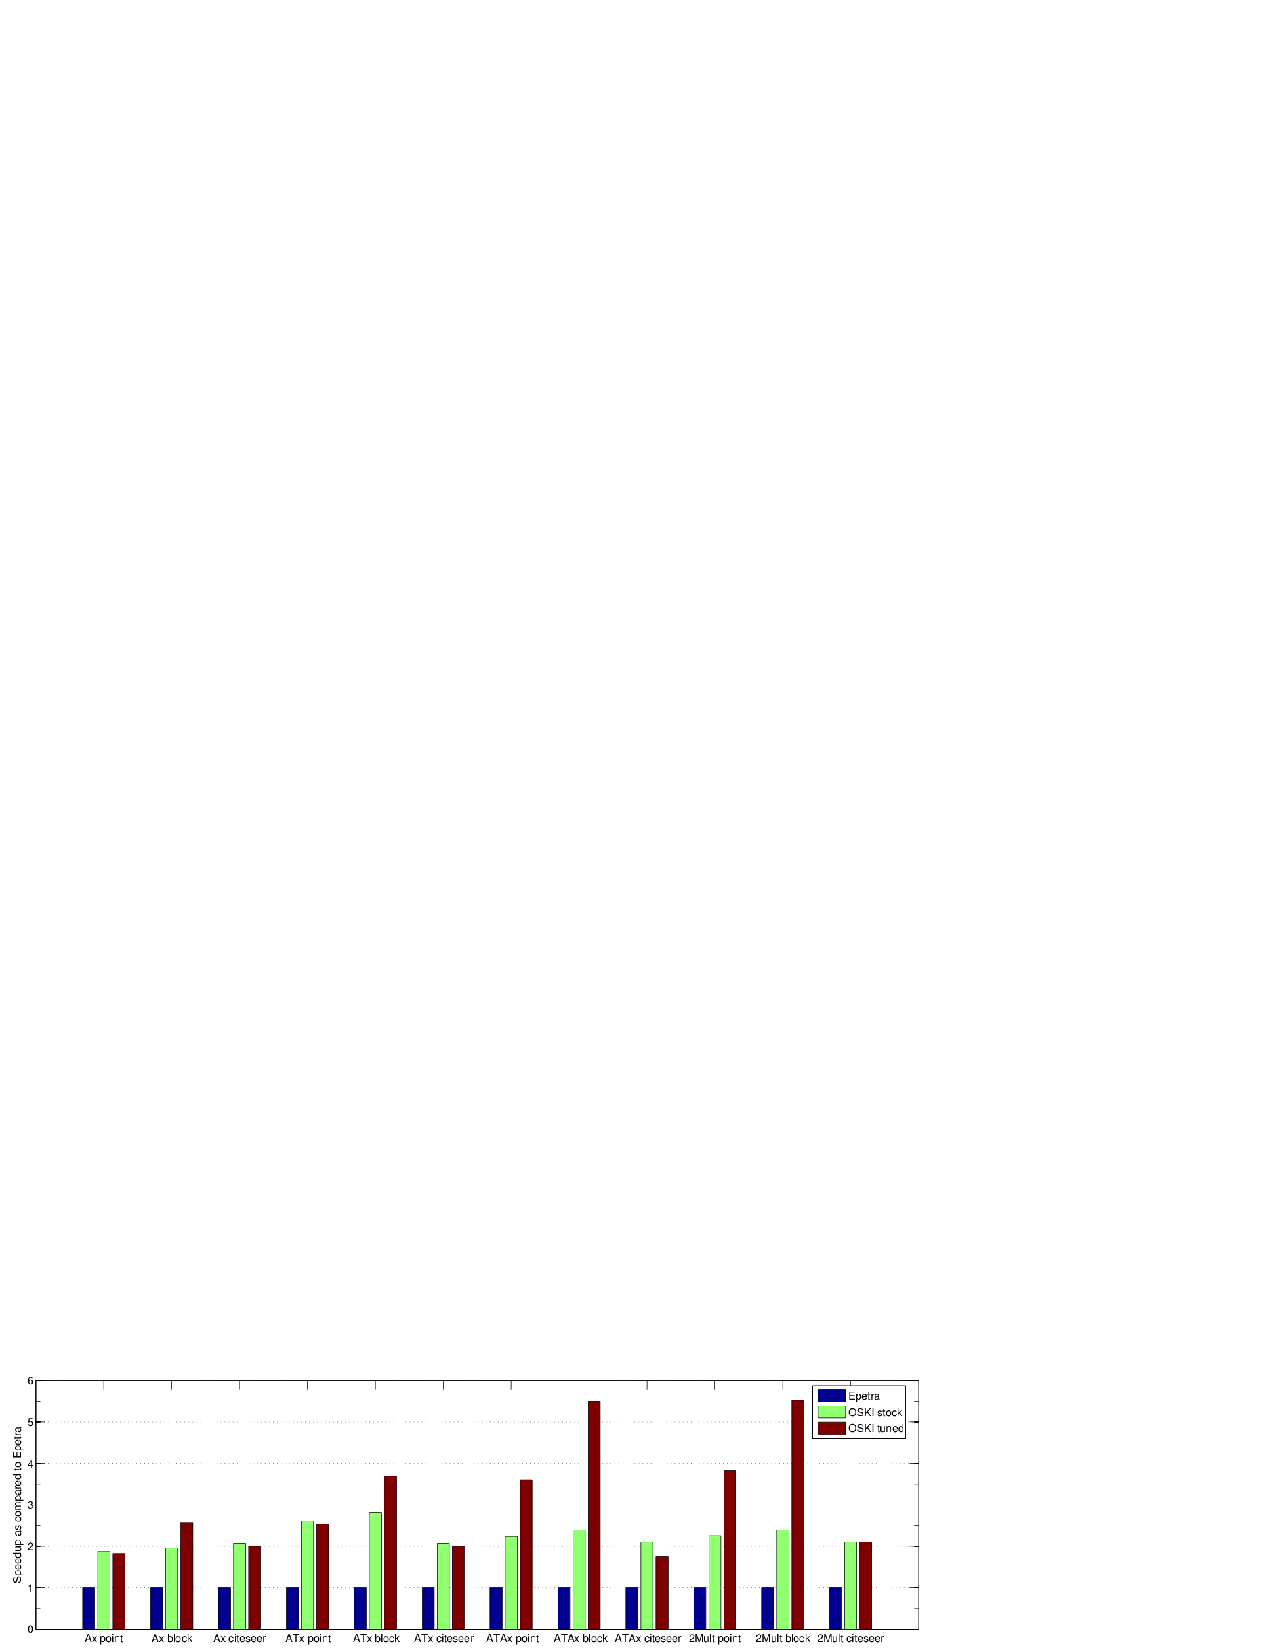
\includegraphics[scale=.8]{./plots/c3serial.pdf}
\caption{Relative performance of Epetra and OSKI in serial on Clovertown.}
\label{IK:fig:C3serial}
\end{center}
\end{figure}
%
\begin{table}[htbp]
\begin{center}
\begin{tabular}{|l|l|l|l|l|}
\hline
Machine & $Ax$ & $A^Tx$ & $A^TA$ & 2Mult \\
\hline
Clovertown & 220/227/55 & 150/154/43 & 178/183/48 & 178/184/48 \\
%barcelona & & & & \\
Niagara & 58.3/69.9/20.7 & 56/66.4/20.3 & 57.1/68.1/20.5 & 57.1/68.1/20.5 \\
\hline
\end{tabular}
\caption{Epetra serial routine speeds in Mflops.  Results are in the form point/block/Citeseer.}
\label{IK:fig:serialnums}
\end{center}
\end{table}

On the Clovertown, OSKI produced large speedups over Epetra for all matrices in serial,
as shown in Figure \ref{IK:fig:C3serial}.
The stock kernels demonstrated speedups of $1.8$ to $2.8$.  Tuning improved the block matrices by about one third
when compared to the stock kernels. The composed algorithms demonstrated even more significant speedups of up to
5.5, when composing and blocking were combined.
Tuning did not improve the runtime of point matrices, except when a composed
kernel was used.  In the
case of the Citeseer matrix, a composed kernel resulted in either no performance gain or performance
degradation.

%\begin{figure}[htbp]
%\begin{center}
%\includegraphics{./plots/barcelonaserial.pdf}
%\caption{Serial results on Barcelona}
%\label{IK:fig:barcelonaserial}
%\end{center}
%\end{figure}

%Barcelona text here when numbers exist.

\begin{figure}[htbp]
\begin{center}
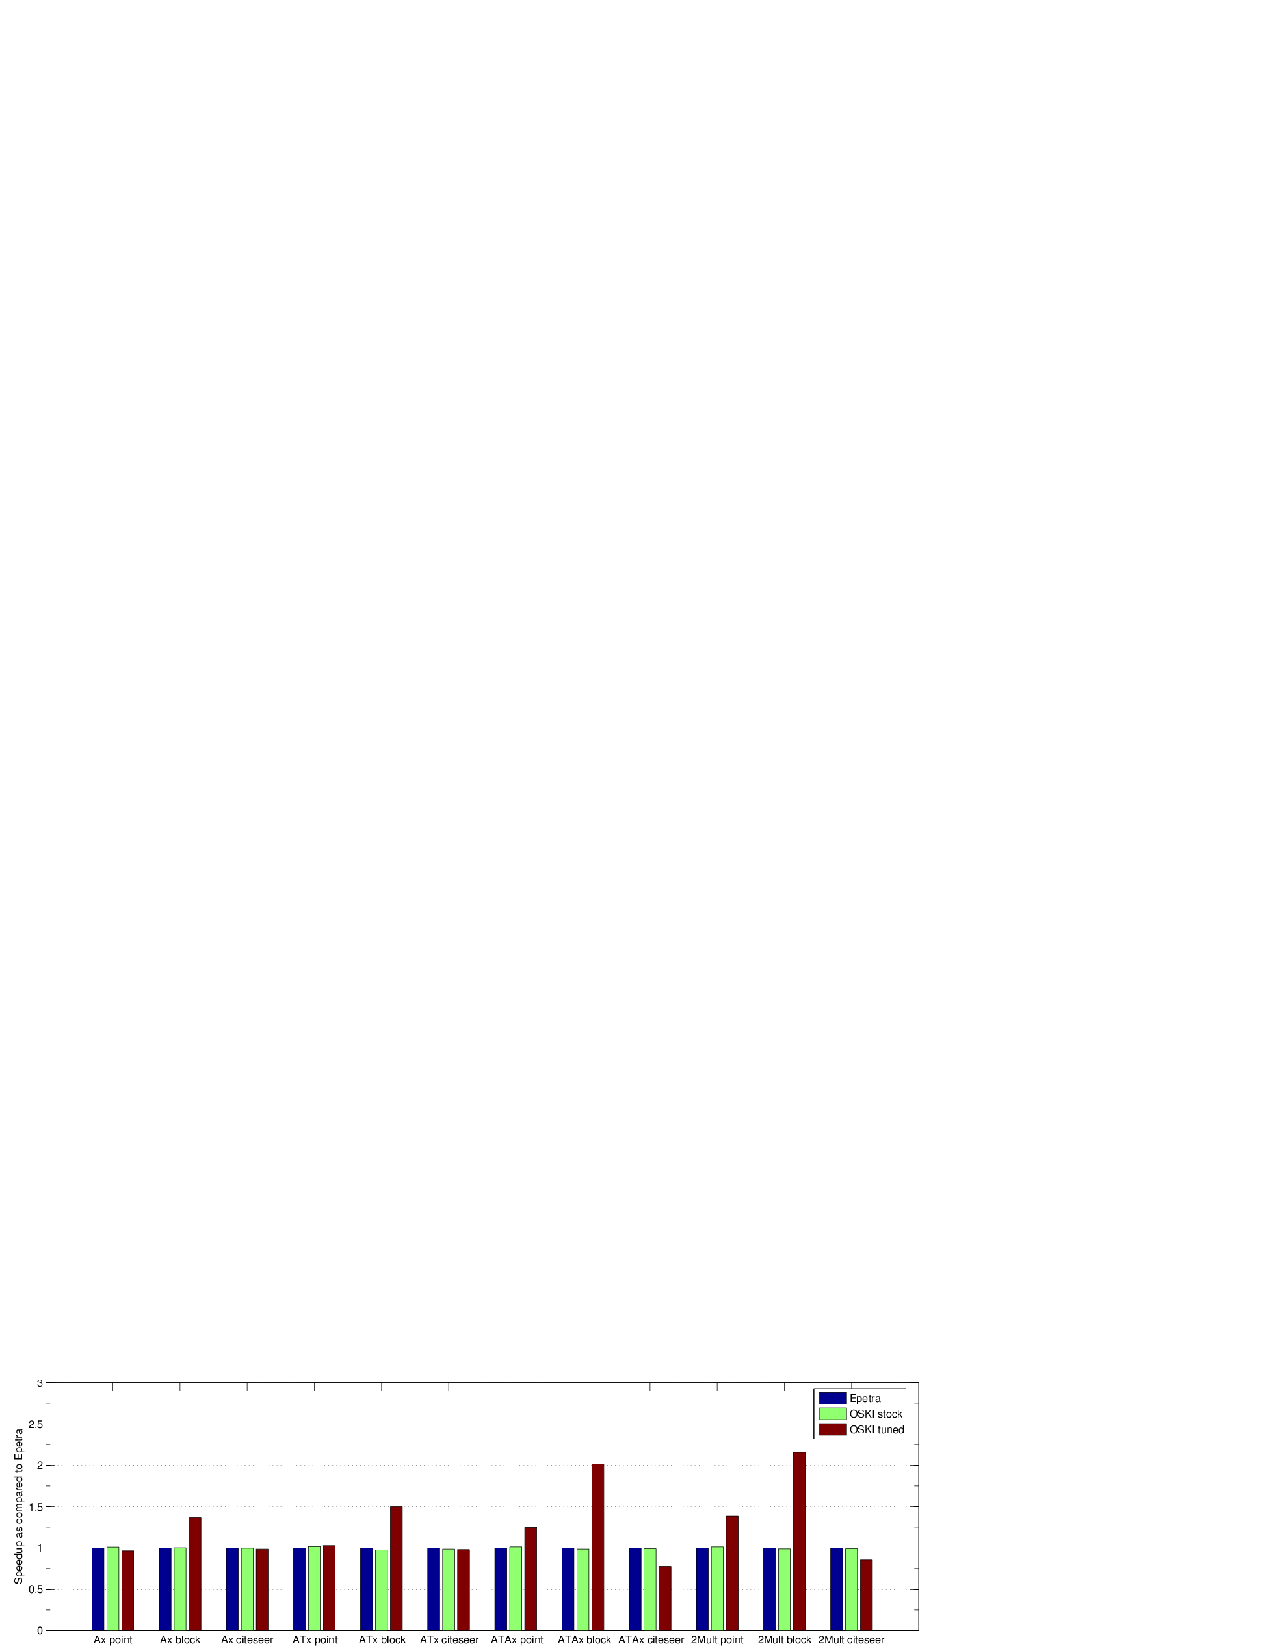
\includegraphics[scale=.8]{./plots/hypnotoadserial.pdf}
\caption{Relative performance of Epetra and OSKI in serial on Niagara.}
\label{IK:fig:hypnotoadserial}
\end{center}
\end{figure}

Figure \ref{IK:fig:hypnotoadserial} shows that
on the Niagara, the stock OSKI and Epetra kernels had roughly the same performance
Tuning for point matrices once again resulted in either no gains or
slight losses. Tuning for block matrices resulted in a one third to one half gain in speed.  Again,
composing increased the speed of all kernels significantly, except for the Citeseer matrix, for which the
OSKI kernels where actually slower.

As expected, the serial tests show that the tuning of point matrices is counterproductive,
except when needed to use composed kernels.
However, tuning of block matrices results in significant speedups through the reduction of indirect addressing.  For the
pseudo random Citeseer matrix, tuning is never beneficial.  This is probably due to either lack of cache-blocking in the composed kernels
 and/or more random access, which create a greater number of cache misses.
% by increasing reuse distances between reads of individual vector elements.
For structured matrices, composing results in a 25\% to 60\% gain over the faster of the stock and tuned kernels.

Even if the tuning gains shown above are large, the amount of time it takes to tune a matrix at runtime is important in determining whether
tuning will result in performance gains.  Tables \ref{IK:fig:tuningcostspoint}, \ref{IK:fig:tuningcostsblock}
and \ref{IK:fig:tuningcostsciteseer} show the cost of tuning and the number of matrix-vector calls needed to amortize that cost for the point, block, and Citeseer matrices, respectively.
 The tuning and retuning costs are expressed in terms of
the number of matrix-vector multiplies that could be performed in the time it takes to tune.
{\it Tuning cost} is the amount of time it takes to tune a matrix the first time, and includes
time to analyze the matrix to determine what optimizations are beneficial.
{\it Retuning cost} is the amount of time it takes to tune the matrix if the optimizations
to be performed are already known.  All comparisons are to the faster of the Epetra and OSKI matrix-vector
multiplies.  The amortize columns show the number of calls to the tuned kernel needed to realize
tuning gains.  When N/A is listed in an amortize column, it is never better to tune
because the tuned kernels are no faster than the untuned kernels.
We note that the tuning cost depends only on the matrix structure, not on the matrix kernel to be
performed.
%
\begin{table}[htbp]
\centering
\begin{tabular}{|l|l|l|l|l|}
\hline
Machine & Tune/Retune & Amortize & Amortize & Amortize \\
 & & $Ax$/Retune & $A^TA$/Retune & 2Mult/Retune \\
\hline
Clovertown & 37.6 / 20.1 & N/A & 48 / 26 & 45 / 24 \\
%Barcelona & & & & \\
Niagara & 22.1 / 12.7 & N/A & 56 / 33 & 40 / 24 \\
\hline
\end{tabular}
\caption{OSKI tuning costs for point matrix.  Cost is equivalent number of matrix-vector multiplications.} \label{IK:fig:tuningcostspoint}
\end{table}

\begin{table}[htbp]
\begin{center}
\begin{tabular}{|l|l|l|l|l|}
\hline
Machine & Tune/Retune & Amortize & Amortize & Amortize \\
 & & $Ax$/Retune & $A^TA$/Retune & 2Mult/Retune \\
\hline
Clovertown & 31.1 / 17.7 & 131 / 75  & 27 / 16 &  28 / 16  \\
%Barcelona & & & & \\
Niagara & 22.5 / 14.1 & 86 / 54 & 22 / 14  & 21 / 13 \\
\hline
\end{tabular}
\caption{OSKI tuning costs for block matrix. Cost is equivalent number of matrix-vector multiplications.}
\label{IK:fig:tuningcostsblock}
\end{center}
\end{table}


\begin{table}[htbp]
\begin{center}
\begin{tabular}{|l|l|l|l|l|}
\hline
Machine & Tune/Retune & Amortize & Amortize & Amortize \\
 & & $Ax$/Retune & $A^TA$/Retune & 2Mult/Retune \\
\hline
Clovertown & 14.5 / 6.7 & N/A & N/A & N/A \\
%Barcelona & & & & \\
Niagara & 11.5 / 5.2 & N/A & N/A & N/A \\
\hline
\end{tabular}
\caption{OSKI tuning costs for Citeseer matrix. Cost is equivalent number of matrix-vector multiplications.}
\label{IK:fig:tuningcostsciteseer}
\end{center}
\end{table}

In many cases, the tuned OSKI kernels are much more efficient than the Epetra and
OSKI stock kernels.
However, the data structure rearrangement required to create an OSKI
kernel is non-trivial. The cost of tunings ranges from 11.5 to 37.6 equivalent matrix-vector multiplies.
It can require as many as 131 subsequent kernel applications to recoup the cost of initial tuning.
However, re-tuning costs are usually slightly over half the cost
of the initial tuning, so saving transformations for later use could be profitable.  Block
matrices require the smallest number of calls to recover tuning costs, and when combined with
composed kernels, this number drops even more.
For point matrices tuning the matrix-vector
multiply is never profitable, but the tuning of composed kernels can be profitable
for structured matrices.

While serial performance is important to application performance, most scientific simulations are
run on parallel machines.  The first level of parallelism is within a single node,
which typically contains one or two multicore processors.  To test the scalability of our
implementation of OSKI, within Epetra, we ran tests on each matrix on 1 to 8 cores of each machine
and also on 1 to 8 threads per core on the Niagara.

\begin{figure}[htbp]
\centering
\subfigure[Clovertown]{
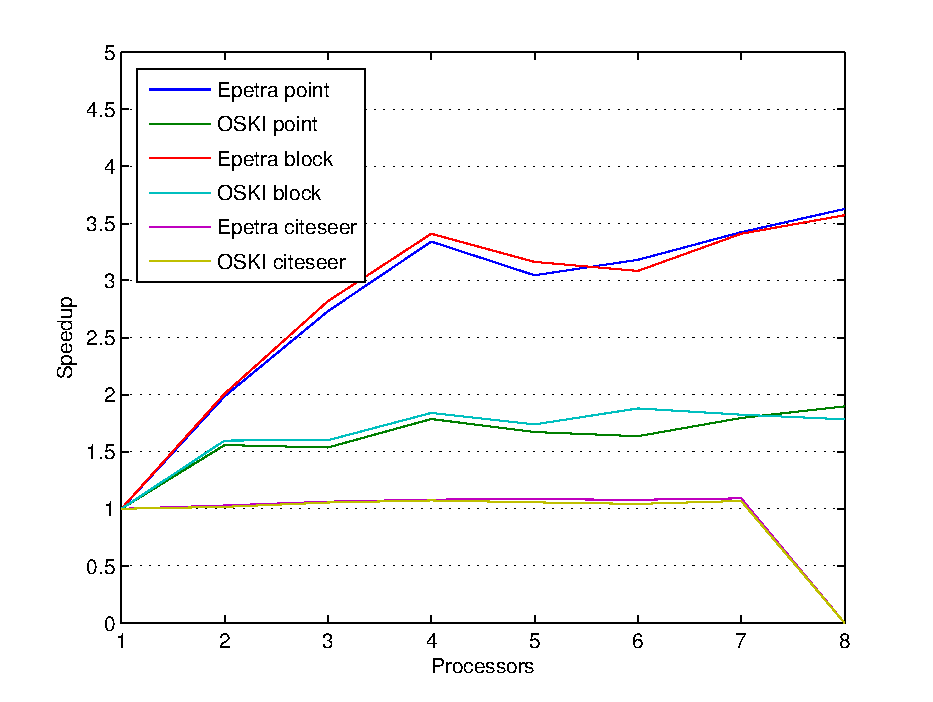
\includegraphics[scale=.39]{./plots/c3scale.pdf}
\label{IK:fig:c3strong}
}
\subfigure[Niagara]{
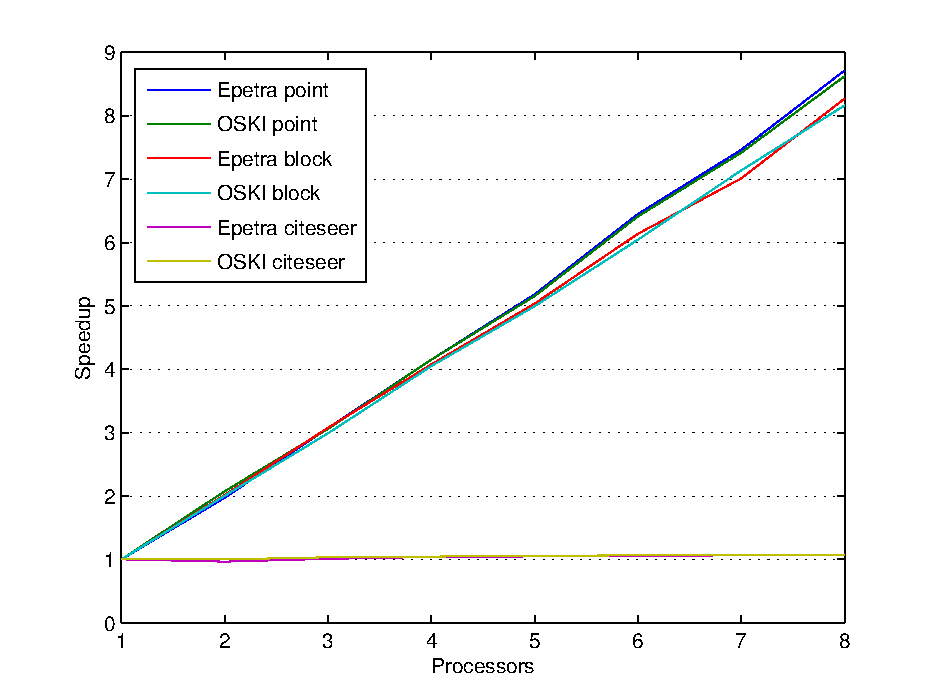
\includegraphics[scale=.39]{./plots/hypnotoadscale.pdf}
\label{IK:fig:hypstrong}
}
\subfigure[Niagara multi-threaded]{
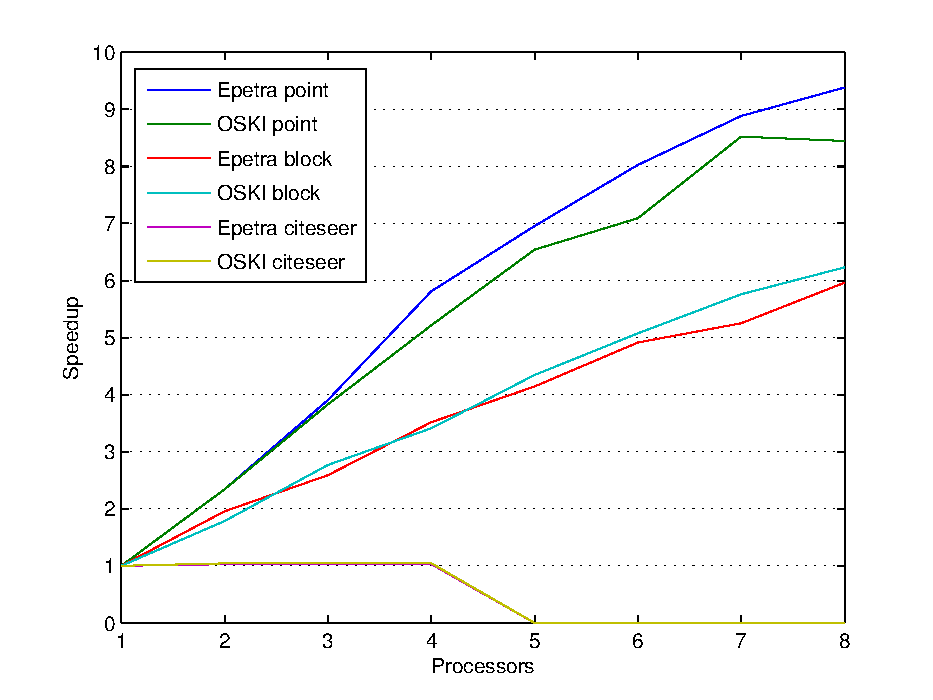
\includegraphics[scale=.39]{./plots/hypnotoadscalebig.pdf}
\label{IK:fig:hypstrongthread}
}
%\caption{Strong scaling results for Clovertown and Niagara processors on top, and Niagara thread scalability on bottom.}
\caption{OSKI matrix-vector multiply strong scaling results.}
\label{IK:fig:strongscale}
\end{figure}

Figures \ref{IK:fig:c3strong}-\ref{IK:fig:hypstrongthread} show the strong scaling of the matrix-vector
kernel for each matrix.  Figure \ref{IK:fig:c3strong}
shows that on the Clovertown that Epetra has better scaling than OSKI. Table
\ref{IK:fig:parrallelnums} shows, however, that the overall performance of OSKI is either comparable or
better to that of Epetra.
The better scaling for Epetra comes from its slower performance in the single processor case, which allows
for more improvement within a limited memory bandwidth situation.
% When most of the matrix fits in cache performance improves faster than
%the number of processors due to increased processing power and decreased memory cost.
For the point matrix, both Epetra and OSKI improve significantly
until each is running at about 735 Mflops on 4 cores.
At this point,  the calculations likely become memory bandwidth limited.
With added processing power, the speeds then improve to slightly under 800 Mflops.
The block matrix results show a similar pattern, with the OSKI block matrix remaining more efficient throughout.
The Citeseer matrix does not scale most likely due to the large amounts of data it needs to exchange, because its
unstructured.  Also it could not be run on 8 processors due to an increasing memory footprint, perhaps due to exchanged data.


\begin{table}[htbp]
\begin{center}
\begin{tabular}{|l|l|l|l|}
\hline
machine & point & block & Citeseer \\
 & Epetra/OSKI & Epetra/OSKI & Epetra/OSKI \\
\hline
Clovertown &  798/782 & 810/1099 & 59.6/122  \\
%barcelona & & & \\
Niagara 1 thread/core & 508/507 & 578/778 & 22.3/22.0\\
Niagara multiple threads/core & 4767/4321 & 3447/4847 & 23.2/23.2 \\
\hline
\end{tabular}
\caption{Epetra and OSKI maximum parallel matrix vector multiply speeds in Mflops.}
\label{IK:fig:parrallelnums}
\end{center}
\end{table}


Figure \ref{IK:fig:hypstrong} shows that on the Niagara both the point and block matrix algorithms scale linearly with the number
of cores.  Essentially, there is enough memory bandwidth to feed each core.  As seen in Figure \ref{IK:fig:hypstrongthread},
 adding more threads per core to the calculating power leads to approximately linear speedup for all matrices.
This begins to tail off at 5 threads for block matrices, and 7 threads for point matrices.  The Citeseer matrix once
again does not scale and becomes too large to run above 32 threads.

Scalability also matters when a matrix is being tuned.  Figures
\ref{IK:fig:c3tuningScal}-\ref{IK:fig:niagthreadtuningScal} show
how well each matrix scales on each machine in terms of tuning cost.  Scaling is usually
linear or slightly better with the number of processors.  This result is expected as tuning is
a local computation with no communication between processors.  As seen in Figure \ref{IK:fig:niagthreadtuningScal},
increasing
the number of threads per Niagara processor initially leads to improved performance, before dropping off at 6
or  more threads per processor.
The dropoff is most likely due to threads competing for processor resources.  Results for the Citeseer matrix were
not shown, as OSKI does not tune its matrix-vector multiply kernel for the Citeseer matrix.  Finally, note
that the retune function demonstrates better scaling than the same tune function in all cases.

\begin{figure}[htbp]
\begin{center}
\subfigure[Clovertown]{
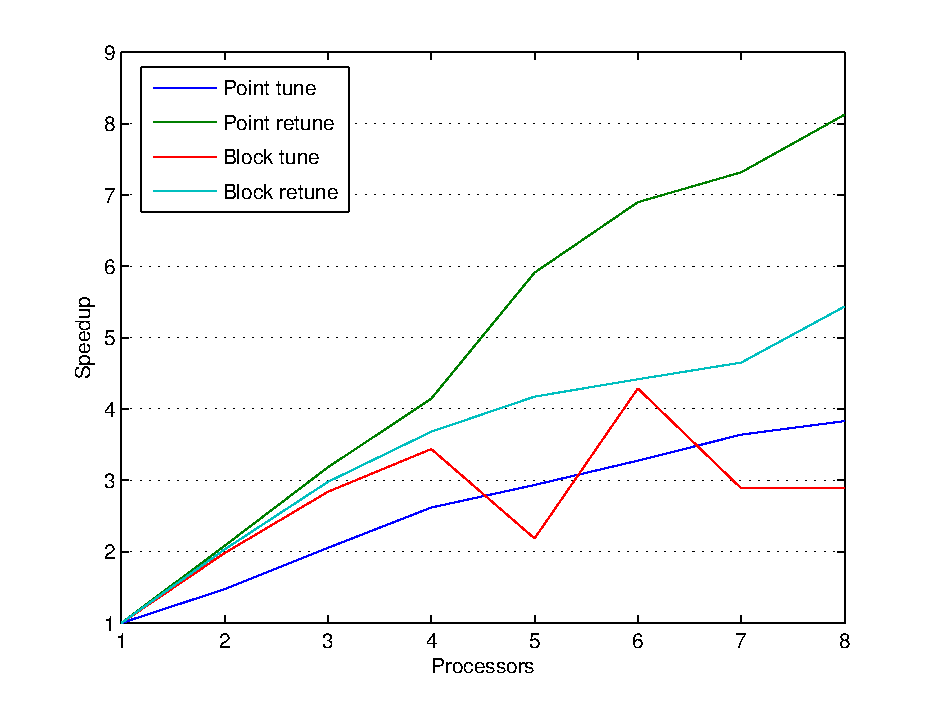
\includegraphics[scale=.4]{./plots/c3tune.pdf}\label{IK:fig:c3tuningScal}}
\subfigure[Niagara single-threaded]{
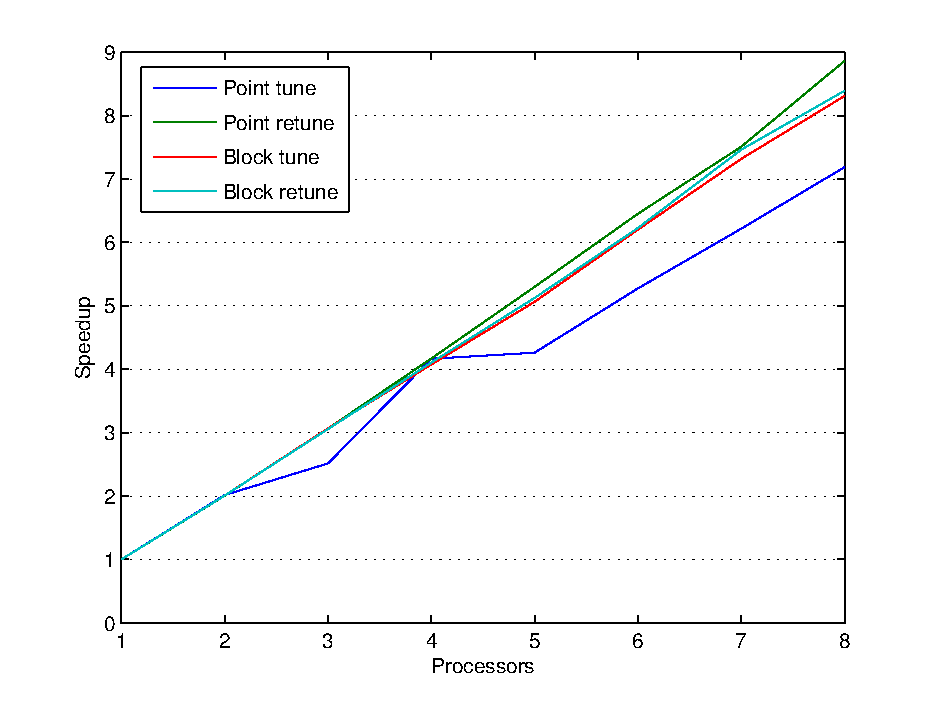
\includegraphics[scale=.4]{./plots/hypnotoadtune.pdf}\label{IK:fig:niagtuningScal}}
\subfigure[Niagara multi-threaded]{
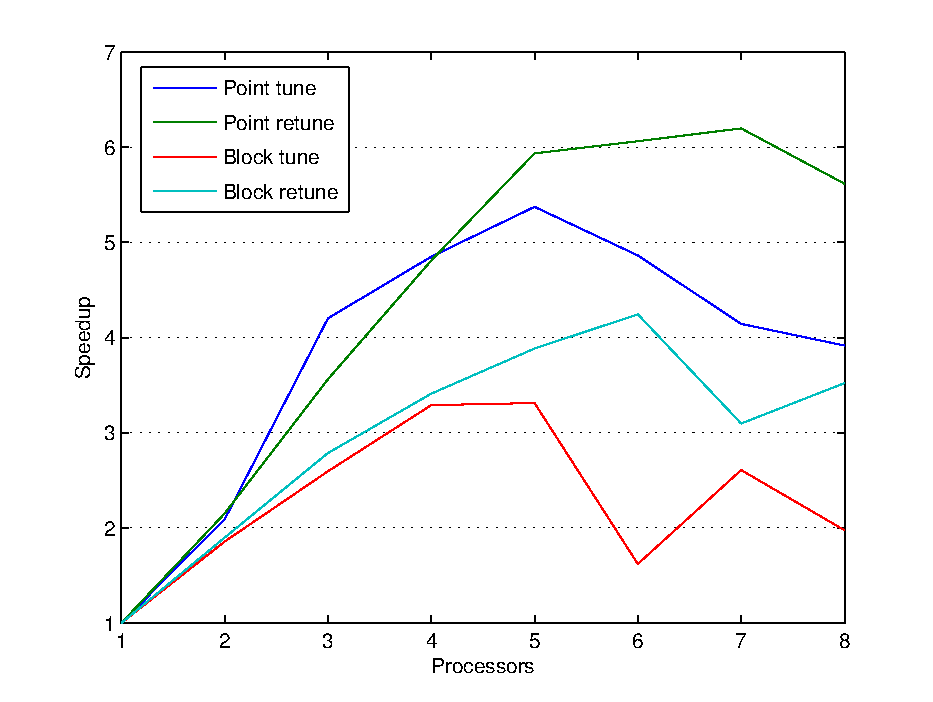
\includegraphics[scale=.4]{./plots/hypnotoadtunebig.pdf}\label{IK:fig:niagthreadtuningScal}}
\caption{Scalability of OSKI tuning.}
% scalability Clovertown and Niagara processor scalability on top and Niagara thread scalability on bottom.}
\label{IK:fig:tuningscale}
\end{center}
\end{figure}

In addition to strong scaling tests, we also ran a weak scaling test on the Niagara.  We used the block
matrix from the 8 thread test case in Table \ref{IK:fig:serialmats}.  Tests were run on 1, 8, 27 and 64 threads.
Results are shown in Figures \ref{IK:fig:weakmatvec}-\ref{IK:fig:weaktune}.  As seen in Figure \ref{IK:fig:weakmatvec}, the OSKI tuned and untuned  matrix-vector
multiplies both scale similarly to Epetra's matrix-vector multiply.  Figure \ref{IK:fig:weakcomposed}, shows that the tuned
composed kernels do not scale well.  The same result was seen for the untuned composed kernels.  For these operations
to be possible there is extra data copying in the wrapping of the serial kernels, which could be the problem.  There could also be
inefficiencies in the code in other places or resource contention on the processor.
%, however, it is not known at this time why this issue is occurring.
Figure \ref{IK:fig:weaktune} shows that re-tuning scales better than tuning as
the problem size grows.

\begin{figure}[htbp]
\begin{center}
\subfigure[MatVec]{
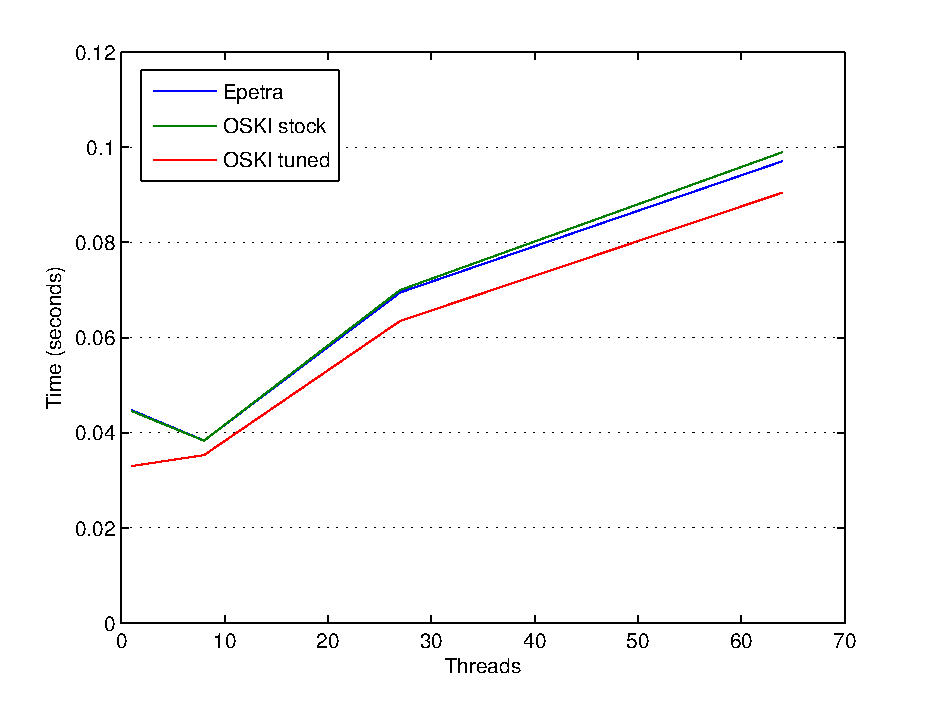
\includegraphics[scale=.4]{./plots/weakmatvec.pdf}\label{IK:fig:weakmatvec}}
\subfigure[Composed]{
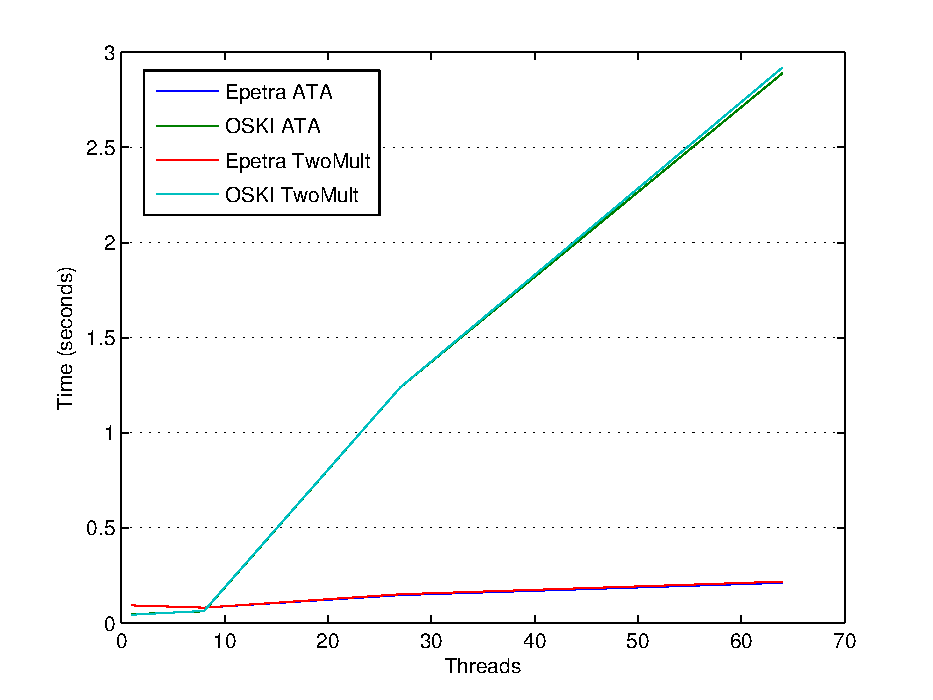
\includegraphics[scale=.4]{./plots/weakcomposed.pdf}\label{IK:fig:weakcomposed}}
\subfigure[Tuning]{
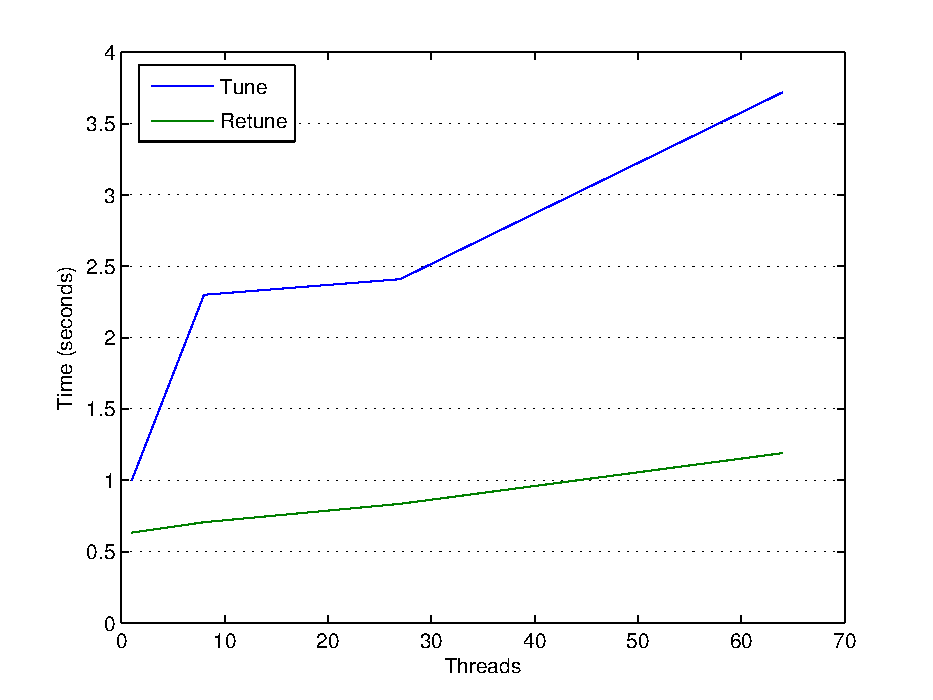
\includegraphics[scale=.4]{./plots/weaktune.pdf}\label{IK:fig:weaktune}}
\caption{Weak scalability of OSKI on Niagara}
% scalability Clovertown and Niagara processor scalability on top and Niagara thread scalability on bottom.}
\label{IK:fig:weakscale}
\end{center}
\end{figure}

%Then maybe a weak scaling numbers that need to be run.
%
%Finally cluster numbers if run.
